\begin{frame}{Λύση: Υπερδειγματοληψία του χάρτη $\Rightarrow$ παραγωγή $2^\nu$ εκτιμήσεων}

  \definecolor{r}{rgb}{0.925 0 0}
  \definecolor{b}{rgb}{0 0.4470 0.7410}

  \noindent\makebox[\linewidth][c]{%
  \begin{minipage}{\linewidth}
    \begin{minipage}{0.3\linewidth}
      \begin{figure}
        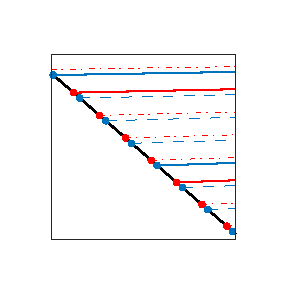
\includegraphics{./figures/slides/ch6/oversampling/false_oversampling_2}
      \end{figure}

      \begin{textblock}{14}(1,4.1)\scriptsize
        \textcolor{b}{$\mathcal{S}_R^{\text{ - -interp}}(\theta)$} \hspace{0.05cm} \textcolor{r}{$\mathcal{S}_V^{\text{ - -oversamp}}(\hat{\theta})$}
      \end{textblock}
      \begin{textblock}{14}(5.7,4.1)\scriptsize
        \textcolor{b}{$\mathcal{S}_R^{\text{ - -interp}}(\theta)$} \hspace{0.05cm} \textcolor{r}{$\mathcal{S}_V^{\text{ - -oversamp}}(\hat{\theta})$}
      \end{textblock}
    \end{minipage}
    %\hfill
    \begin{minipage}{0.3\linewidth}
      \begin{figure}
        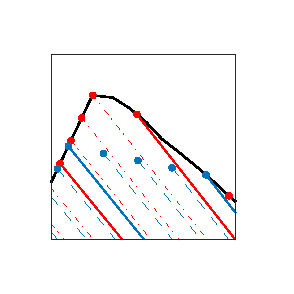
\includegraphics{./figures/slides/ch6/oversampling/false_oversampling_4}
      \end{figure}
    \end{minipage}
    %\hfill
    \begin{minipage}{0.3\linewidth}
      \begin{figure}
        \animategraphics[autoplay,loop]{2}{./figures/slides/ch6/oversampling/correct_oversampling_}{1}{4}
      \end{figure}

      \begin{textblock}{14}(10.4,4.1) \scriptsize
        \textcolor{b}{$\mathcal{S}_R(\theta)$} \hspace{0.25cm} \textcolor{r}{$\mathcal{S}_V(\hat{\theta} + \{0...2^{\nu_{\max}}$$-$$1\} \cdot \dfrac{\gamma}{2^{\nu_{\max}}})$}
      \end{textblock}

      \begin{textblock}{14}(10.4,11.1)
        $\phi^\prime = \dfrac{\phi}{2^{\nu_{\max}}} \leq \dfrac{\gamma}{2^{1+\nu_{\max}}}$
      \end{textblock}
    \end{minipage}
  \end{minipage}
  }

\note{\footnotesize
Η γνώμη μου είναι ότι ο μόνος τρόπος για τη μείωση του γωνιακού σφάλματος χωρίς
  την ακούσια εισαγωγή σφαλμάτων είναι η υπερδειγματοληψία μόνο του χάρτη. Αυτό
  σημαίνει ότι αν θέλουμε να ελαττώσουμε το σφάλμα κατά 2 εις την ν φορές,
  αρκεί να υπολογίσουμε 2 εις την ν εικονικές σαρώσεις με μέγεθος ίσο με την
  πραγματική σάρωση, να ευθυγραμμίσουμε την κάθε μία με αυτήν, και να
  εκτιμήσουμε ποιά από τις 2 εις την ν εκτιμήσεις εμφανίζει το μικρότερο
  σφάλμα.  Οπότε τώρα εμφανίζεται μπροστά μας άλλο πρόβλημα.  Δεδομένου ενός
  συνόλου εκτιμήσεων οι οποίες όλες έχουν την ίδια θέσης αλλά
  διαφορετικό προσανατολισμό, ποιά απο αυτές εμφανίζει το
  χαμηλότερο σφάλμα προσανατολισμού?}

\end{frame}
